\section{Results}\label{sec:results}
\subsection{A positive pipeline contrast required no runtime packet}
The original visual confirmation completed all 500 scheduled environments. The packet-input/full-action policy lost reward against local continuation on both tasks (Table~\ref{tab:visual}). A separate audit reproduced all saved choices and reward means. These are results of the frozen selectors, not the quality of every possible expert intervention.
\begin{table}[tb]
\centering\small
\caption{Original visual confirmation. $L/P$: local/packet input; $C/F$: local/full action set; $R$: reject. All are separately fitted frozen variants. $n=250$ paired environments/task; approximate 99.5833\% intervals.}\label{tab:visual}
\begin{tabular}{llrr}
\toprule Task & Contrast & Mean & Interval\\
\midrule
Push & $P,C-L,C$ & +0.007 & [-0.078, +0.144]\\
Push & $P,F-P,C$ & +0.139 & [-0.005, +0.355]\\
Push & $P,F-R$ & -0.365 & [-0.719, -0.050]\\
PickPlace & $P,C-L,C$ & +0.735 & [+0.294, +1.216]\\
PickPlace & $P,F-P,C$ & -0.636 & [-1.080, -0.230]\\
PickPlace & $P,F-R$ & -0.636 & [-1.080, -0.230]\\
\bottomrule
\end{tabular}
\end{table}


The decisive counterexample is PickPlace's $P,C-L,C$ difference: $+0.735$ with approximate interval $[0.294,1.216]$. Its winning $P,C$ predictor is identically zero and rejects in all 250 environments, producing the same trajectories as local continuation (Fig.~\ref{fig:visual}). Its validation MSE is $1.42955\times10^{-13}$ \emph{higher} than the best nonzero candidate, within the predeclared $10^{-12}$ tie tolerance. It is a tie-selected null, not clear validation superiority. Proposition~\ref{prop:null} certifies that this deployed policy does not require the returned packet. The positive contrast is therefore insufficient to attribute value to newly returned information. Forced queries still occurred; no acquisition saving was measured.

\begin{figure}[tb]\centering
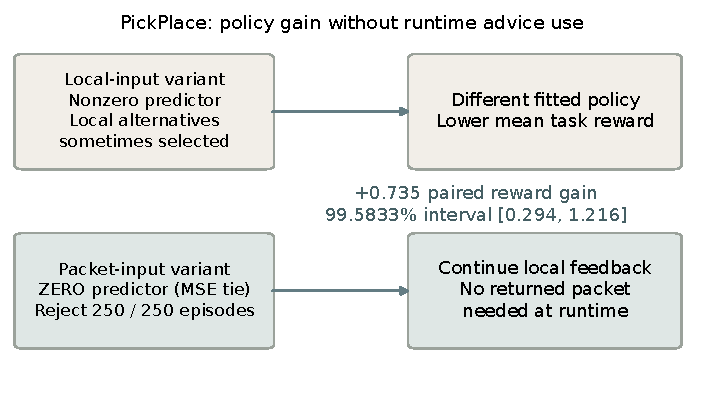
\includegraphics[width=\textwidth]{figures/null_counterexample.pdf}
\caption{PickPlace's positive input-labelled contrast compiles to continued local feedback. The zero predictor wins a validation tie and never accepts an intervention. The performance gap is real for these separately fitted pipelines, but does not establish runtime message value.}\label{fig:visual}
\end{figure}

The original full-policy losses were mostly assigned to selected local alternatives: on Push, 149 local selections contributed $-0.364$, 17 source selections about $-0.001$, and 84 rejects zero to the overall difference. PickPlace's 170 local and 80 source selections contributed $-0.652$ and $+0.016$. This descriptive accounting does not identify effects within selected strata or validate deleting local options after testing. An elapsed-aligned source suffix had positive descriptive differences against reject on both tasks; learned-router loss is not failure of every source action.

\subsection{Direct visual and state message-channel outcomes}\label{sec:channelresults}
The visual bridge completes 60 fresh nonzero-delay PickPlace environments with the original frozen actors and receivers. The nonzero $P,F$ gate changes option after refresh in 10/60 cases; complete action sequences change in 28/60. Its refresh-minus-stale reward difference is $-0.1428$ with approximate 98.3333\% interval $[-0.4932,0.2285]$, leaving a positive refresh benefit unresolved. Stale-minus-absence is $-0.5180$ $[-1.1557,0.0521]$; fresh-minus-absence is $-0.6608$ $[-1.2486,-0.0836]$. Thus the fresh implementation performs below the specified reject fallback in this cohort, while the fresh/stale comparison does not establish benefit or equivalence.

The original null $P,C$ receiver continues to reject under all three channels, with identical trajectories. By contrast, the local-input/full-action receiver changes no option but changes actions in 19/60 cases. This directly demonstrates gate versus actuation dependence in the original visual setting. The $P,C$ counterexample and $P,F$ channel estimate remain different frozen receivers within one actor system, not interchangeable estimands.

The full packet receiver's any-success is 83.3\% stale, 80.0\% fresh and 88.3\% absent; terminal-success is 60.0\%, 61.7\% and 58.3\%. These descriptive endpoints need not rank channels identically. All 177 distinct main-cohort plans retain full trajectories; six separate zero-delay identities and two engineering cases are excluded. Independent replay regenerates request/arrival source packets and features, and every reject tail is checked. The result concerns one task and one trained visual system with its unchanged delay-indexed decoder.

The state study separately executed all 180 fresh environments. For its full packet policy, refreshing changed mean reward by $+0.037667$ on Drawer and $+0.038542$ on Door; both primary intervals include zero (Table~\ref{tab:channel}). This leaves a positive refresh benefit unresolved. It does not prove advice inefficacy or equivalence. Button is different: its selected zero policies structurally reject under all channels. Under the declared absence-to-reject wrapper, stale delivery reduces reward on Drawer and Door. That availability contrast includes the specific fallback and does not establish that expert information is generally harmful.
\begin{table}[tb]\centering\small
\caption{Fixed full packet receiver: primary native reward channel effects. PickPlace uses one frozen visual system and 60 nonzero-delay environments (98.3333\% intervals, family of three). State rows use 60 environments/task including zero delay and five frozen critics (99.5833\%, original family of 12). $S/F/E$ denote stale/fresh/absent; absence invokes the fixed reject wrapper. These distinct regimes are not pooled. Button zeros are structural.}\label{tab:channel}
\setlength{\tabcolsep}{4pt}\begin{tabular}{llrr}\toprule Task / observation & Contrast & Mean & Interval\\\midrule
PickPlace / RGB & $F-S$ & -0.1428 & [-0.4932, +0.2285]\\
PickPlace / RGB & $S-E$ & -0.5180 & [-1.1557, +0.0521]\\
PickPlace / RGB & $F-E$ & -0.6608 & [-1.2486, -0.0836]\\
Drawer / state & $F-S$ & +0.0377 & [-0.0232, +0.2076]\\
Drawer / state & $S-E$ & -0.0756 & [-0.2513, -0.0117]\\
Drawer / state & $F-E$ & -0.0380 & [-0.0728, -0.0127]\\
Door / state & $F-S$ & +0.0385 & [-0.1016, +0.2079]\\
Door / state & $S-E$ & -0.1026 & [-0.2906, -0.0004]\\
Door / state & $F-E$ & -0.0640 & [-0.2148, +0.0003]\\
Button / state & $F-S$ & +0.0000 & [+0.0000, +0.0000]\\
Button / state & $S-E$ & +0.0000 & [+0.0000, +0.0000]\\
Button / state & $F-E$ & +0.0000 & [+0.0000, +0.0000]\\
\bottomrule\end{tabular}\end{table}


Choice and command dependence differ. Among the 300 state environment/critic records per task, $P,F$ changes option under refresh in 62 Drawer and 57 Door records, but complete actions change in 142 and 159. The local-input/full-action selector changes \emph{no} option while actions change in 115 and 114 records: a fixed named source option executes different message values. A gate-only audit misses this path. Door's $P,C$ changes choices and actions in 90/300 records. These are sampled-input diagnostics, not global certificates.

State any-success is identical across channels: 100\% Drawer/Button and 95\% Door. Door terminal-success is 0\%. Only about 30 of 500 steps satisfy its native coordinate-band criterion. Figure~\ref{fig:door-time} shows this transient success alongside sustained shaped reward; flag loss alone does not identify door reclosure. Full duration data and post-hoc nonzero-delay uncertainty are in Online Resource 1. These endpoints answer different questions; reward is not a universally superior objective.


\begin{figure}[tb]\centering
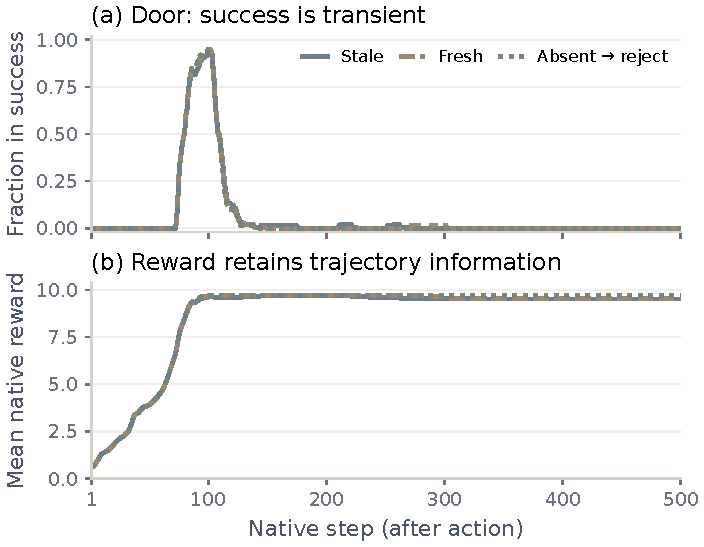
\includegraphics[width=\textwidth]{figures/door_temporal.pdf}
\caption{Door success and native reward under stale, fresh and absent-message channels. Means retain all 60 environments and five frozen $P,F$ critics with environment-equal weighting. Brief success-band occupancy explains the 95\% ever-success/0\% terminal-success discrepancy, while shaped reward remains high. No trajectory selection or timewise inference is used. Full descriptive data are in Online Resource 1.}\label{fig:door-time}
\end{figure}

\subsection{Headroom separates opportunity from harmful selection}\label{sec:headroomresults}
Finite-pool diagnosis reveals two regimes (Table~\ref{tab:headroom}). The visual all-option subset has substantial headroom: 1.285 Push and 1.630 PickPlace, with selector regret 0.978 and 2.396. Some source option exceeds reject by 0.25 in 43.3\% and 36.7\% of the 30 system--environment records/task. Lack of useful candidate actions alone cannot explain these visual failures. However, source-exclusive headroom above the best local option averages only 0.0203 and 0.0913: most available improvement is shared with local alternatives.
\begin{table}[tb]\centering\small
\caption{Distinct finite-pool regimes under stale messages. $H$: full headroom; $H_E$: positive best-source gain; $X$: source-exclusive headroom over the best local option; $G$: full packet selector regret. Visual rows use ten shared initial environments/task across three systems; state rows use 60 environments/task and five critics. No rows are pooled, and no oracle is deployable.}\label{tab:headroom}\label{tab:visualoracle}
\begin{tabular}{llrrrr}\toprule Task & Observation & $H$ & $H_E$ & $X$ & $G$\\\midrule
Push & RGB+robot & 1.2850 & 0.3733 & 0.0203 & 0.9775\\
PickPlace & RGB+robot & 1.6298 & 0.8230 & 0.0913 & 2.3963\\
Drawer & State & 0.00657 & 0.00404 & 0.00150 & 0.08222\\
Door & State & 0.00073 & 0.00048 & 0.00042 & 0.10331\\
Button & State & 0.00026 & 0.00025 & 0.00025 & 0.00026\\\bottomrule
\end{tabular}
\end{table}


The state pool instead offers little average improvement: full-pool headroom is below 0.008 even with refresh, and no stale source option improves by more than 0.25 in any environment. Stale-channel regret on Drawer/Door is much larger than available headroom. Only 24.1\%/2.5\% of selected source actions improve on reject. Drawer source selections contribute $-0.076528$ to the overall $-0.075647$ difference, unlike the local-alternative losses in the original visual cohort. Candidate opportunity and failure mechanism therefore differ by regime; neither diagnosis transfers automatically between them.

The identity $U_\pi-U_R=H-G$ explains how limited opportunity and selection loss coexist. Headroom uses future outcomes and is not deployable performance, nor an information-value upper bound: messages could help select local options. Lowering the state acceptance threshold from $10^{-8}$ to zero changes no recorded choice, so that small threshold does not explain these decisions. State/time strata are descriptive and mix remaining horizon, task state and request time; they do not uniquely identify prediction error or validate a new selector. Full diagnostics remain in Online Resource 1.

\subsection{Complete visual training variation leaves benefit unresolved}\label{sec:fullseedresults}
Three complete systems were evaluated on 100 shared independent initial environments, yielding 300 logical arrival cases plus separate reset-source trajectories. All 1,200 fitted-cell decisions and saved reward means were reproduced, with unchanged model hashes. The full packet policy's difference from reject is $+0.068$ on Push and $-0.382$ on PickPlace; their approximate 99.1667\% intervals cross zero (Table~\ref{tab:fullseeds}). None of the six primary contrasts has a positive lower bound.
\begin{table}[tb]\centering\small
\caption{Complete visual training replication: three independently trained systems, each with a 15,000-update ACT budget, all four local heads and separately fitted arrival critics. Fifty initial environments/task are shared across seeds. These are pipeline contrasts with approximate 99.1667\% crossed-bootstrap intervals (six-contrast family), conditional on the common demonstration corpus and development schedule.}\label{tab:fullseeds}
\begin{tabular}{llrr}\toprule Task & Contrast & Mean & Interval\\\midrule
Push & $P,C-L,C$ & -0.009 & [-0.427, +0.260]\\
Push & $P,F-P,C$ & +0.206 & [-0.066, +0.861]\\
Push & $P,F-R$ & +0.068 & [-0.593, +0.722]\\
PickPlace & $P,C-L,C$ & +0.426 & [-0.367, +1.600]\\
PickPlace & $P,F-P,C$ & -0.361 & [-1.526, +0.000]\\
PickPlace & $P,F-R$ & -0.382 & [-1.500, +0.319]\\
\bottomrule\end{tabular}\end{table}


The PickPlace input contrast is $+0.426$ $[-0.367,1.600]$, qualifying transfer of the original positive pipeline result across training randomness. Seed 0's exact null $P,C$ again rejects all 50 new cases; the other 23 input/action/task/seed cells are nonzero. These correlated cells do not estimate a population null-selection frequency. Push seed 1 has a $+0.379$ full-policy point difference with all 50 interventions assigned to local alternatives; its nonzero packet gate could still use messages to route among them. Absence of source actuation is not independence. Per-seed contrasts and complete-source competence, including all weak outcomes, are retained only in Online Resource 1, Tables S8--S9. The systems share data, pretraining and development arrangements, so this is conditional training variation, not cross-dataset generalization.

\subsection{Generation-time decoding and the frozen selector differ}\label{sec:decoderresults}
Matching generation time improves the predefined fresh 48-step chunk relative to applying its old delay offset: the paired mean gain is 0.579 (Table~\ref{tab:decoder}). This establishes an execution-index effect for that fixed option in the new cohort. Its time-matched fresh versus stale difference remains unresolved, as does its descriptive advantage over continued local control ($+0.120$, 95\% interval $[-0.187,0.433]$). Improvement in this decoder comparison does not by itself establish a useful refresh channel or an overall advice advantage.
\begin{table}[tb]\centering\small
\caption{Independent generation-time decoding control: four primary reward contrasts on 60 new environments. Time uses generation age; legacy uses request delay. Stale decoding is identical for both. Approximate 98.75\% stratified paired-bootstrap intervals retain the four-contrast family. Fixed48 applies the predefined source suffix on every environment; the frozen gate uses unchanged choices across fresh decoders. This study does not alter the original channel estimates.}\label{tab:decoder}
\setlength{\tabcolsep}{3pt}\begin{tabular}{llrr}\toprule Receiver & Contrast & Mean & Interval\\\midrule
Fixed48 & Fresh: time $-$ legacy & +0.579 & [+0.173, +0.997]\\
Fixed48 & Time-fresh $-$ stale & +0.149 & [-0.204, +0.516]\\
Frozen $P,F$ & Fresh: time $-$ legacy & -0.030 & [-0.298, +0.192]\\
Frozen $P,F$ & Time-fresh $-$ stale & -0.188 & [-0.541, +0.116]\\
\bottomrule\end{tabular}\end{table}


The frozen $P,F$ gate responds differently. It chooses a suffix in 24/60 environments (21 for 48 steps and three for 16), so time matching changes 24 action sequences while changing no fresh-channel choice. Its mean decoder effect is $-0.030$, with a primary interval crossing zero. Local-option selections are unaffected. The fixed option's overall gain therefore does not transfer automatically to the gate's selected states and intervention lengths. The gate still predicts legacy-execution gains; this study does not test learning or recalibrating it for the new rule. Complete channel/decoder outcomes, success endpoints and index checks are in Online Resource 1.

These new results qualify a practical reading of the earlier channel test: literal replacement in the legacy receiver and generation-matched execution answer different questions. We retain both, with separate environments, receivers and inference families. The positive fixed-chunk decoder result is not used to relabel the original refresh effect or the packet-independent $+0.735$ counterexample.

\subsection{Supporting analyses bound rather than erase the counterexample}\label{sec:toleranceresults}
The independent critic-data curve uses 7/14/28 nested training episodes with fixed validation. All 24 selected models are nonzero. At 28 episodes, $P,F-R$ is $+0.013$ on Push and $-0.087$ on PickPlace; neither interval establishes benefit. The single nested draw does not prove that more data or a different selector cannot help.

Selection tolerance and deployment threshold have different roles. Across the same 100 development resplits, PickPlace $P,C$ selects zero in 13/14/17/19/19 cases at tie tolerances $0/10^{-14}/10^{-12}/10^{-10}/10^{-8}$. Null prevalence depends on the selection rule and split. The original $+0.735$ estimate is conditional on that rule; the strict-MSE alternative is a different policy whose test effect was not measured. The frozen zero policy's exact independence, and the logical failure of pipeline gain to establish channel value, do not require zero to be commonly selected.

The 360-environment state stress suite varies delay, frequency and noise. It establishes no positive packet/local-input advantage; full policies lose reward on Drawer/Door while Button structurally rejects. Door's zero-packet probe changes 70.9\% of $P,C$ choices, but lacks rerolled outcomes and may be outside training support. It is sensitivity evidence only. All primary contrasts, condition tables, curves, tolerance grids and historical source-budget results remain in Online Resource 1. None is used for test-driven retuning.
